


% Header, overrides base

    % Make sure that the sphinx doc style knows who it inherits from.
    \def\sphinxdocclass{article}

    % Declare the document class
    \documentclass[letterpaper,10pt,english]{/usr/lib/python2.7/site-packages/sphinx/texinputs/sphinxhowto}

    % Imports
    \usepackage[utf8]{inputenc}
    \DeclareUnicodeCharacter{00A0}{\\nobreakspace}
    \usepackage[T1]{fontenc}
    \usepackage{babel}
    \usepackage{times}
    \usepackage{import}
    \usepackage[Bjarne]{/usr/lib/python2.7/site-packages/sphinx/texinputs/fncychap}
    \usepackage{longtable}
    \usepackage{/usr/lib/python2.7/site-packages/sphinx/texinputs/sphinx}
    \usepackage{multirow}

    \usepackage{amsmath}
    \usepackage{amssymb}
    \usepackage{ucs}
    \usepackage{enumerate}

    % Used to make the Input/Output rules follow around the contents.
    \usepackage{needspace}

    % Pygments requirements
    \usepackage{fancyvrb}
    \usepackage{color}
    % ansi colors additions
    \definecolor{darkgreen}{rgb}{.12,.54,.11}
    \definecolor{lightgray}{gray}{.95}
    \definecolor{brown}{rgb}{0.54,0.27,0.07}
    \definecolor{purple}{rgb}{0.5,0.0,0.5}
    \definecolor{darkgray}{gray}{0.25}
    \definecolor{lightred}{rgb}{1.0,0.39,0.28}
    \definecolor{lightgreen}{rgb}{0.48,0.99,0.0}
    \definecolor{lightblue}{rgb}{0.53,0.81,0.92}
    \definecolor{lightpurple}{rgb}{0.87,0.63,0.87}
    \definecolor{lightcyan}{rgb}{0.5,1.0,0.83}

    % Needed to box output/input
    \usepackage{tikz}
        \usetikzlibrary{calc,arrows,shadows}
    \usepackage[framemethod=tikz]{mdframed}

    \usepackage{alltt}

    % Used to load and display graphics
    \usepackage{graphicx}
    \graphicspath{ {figs/} }
    \usepackage[Export]{adjustbox} % To resize

    % used so that images for notebooks which have spaces in the name can still be included
    \usepackage{grffile}


    % For formatting output while also word wrapping.
    \usepackage{listings}
    \lstset{breaklines=true}
    \lstset{basicstyle=\small\ttfamily}
    \def\smaller{\fontsize{9.5pt}{9.5pt}\selectfont}

    %Pygments definitions
    
\makeatletter
\def\PY@reset{\let\PY@it=\relax \let\PY@bf=\relax%
    \let\PY@ul=\relax \let\PY@tc=\relax%
    \let\PY@bc=\relax \let\PY@ff=\relax}
\def\PY@tok#1{\csname PY@tok@#1\endcsname}
\def\PY@toks#1+{\ifx\relax#1\empty\else%
    \PY@tok{#1}\expandafter\PY@toks\fi}
\def\PY@do#1{\PY@bc{\PY@tc{\PY@ul{%
    \PY@it{\PY@bf{\PY@ff{#1}}}}}}}
\def\PY#1#2{\PY@reset\PY@toks#1+\relax+\PY@do{#2}}

\expandafter\def\csname PY@tok@gd\endcsname{\def\PY@tc##1{\textcolor[rgb]{0.63,0.00,0.00}{##1}}}
\expandafter\def\csname PY@tok@gu\endcsname{\let\PY@bf=\textbf\def\PY@tc##1{\textcolor[rgb]{0.50,0.00,0.50}{##1}}}
\expandafter\def\csname PY@tok@gt\endcsname{\def\PY@tc##1{\textcolor[rgb]{0.00,0.27,0.87}{##1}}}
\expandafter\def\csname PY@tok@gs\endcsname{\let\PY@bf=\textbf}
\expandafter\def\csname PY@tok@gr\endcsname{\def\PY@tc##1{\textcolor[rgb]{1.00,0.00,0.00}{##1}}}
\expandafter\def\csname PY@tok@cm\endcsname{\let\PY@it=\textit\def\PY@tc##1{\textcolor[rgb]{0.25,0.50,0.50}{##1}}}
\expandafter\def\csname PY@tok@vg\endcsname{\def\PY@tc##1{\textcolor[rgb]{0.10,0.09,0.49}{##1}}}
\expandafter\def\csname PY@tok@m\endcsname{\def\PY@tc##1{\textcolor[rgb]{0.40,0.40,0.40}{##1}}}
\expandafter\def\csname PY@tok@mh\endcsname{\def\PY@tc##1{\textcolor[rgb]{0.40,0.40,0.40}{##1}}}
\expandafter\def\csname PY@tok@go\endcsname{\def\PY@tc##1{\textcolor[rgb]{0.53,0.53,0.53}{##1}}}
\expandafter\def\csname PY@tok@ge\endcsname{\let\PY@it=\textit}
\expandafter\def\csname PY@tok@vc\endcsname{\def\PY@tc##1{\textcolor[rgb]{0.10,0.09,0.49}{##1}}}
\expandafter\def\csname PY@tok@il\endcsname{\def\PY@tc##1{\textcolor[rgb]{0.40,0.40,0.40}{##1}}}
\expandafter\def\csname PY@tok@cs\endcsname{\let\PY@it=\textit\def\PY@tc##1{\textcolor[rgb]{0.25,0.50,0.50}{##1}}}
\expandafter\def\csname PY@tok@cp\endcsname{\def\PY@tc##1{\textcolor[rgb]{0.74,0.48,0.00}{##1}}}
\expandafter\def\csname PY@tok@gi\endcsname{\def\PY@tc##1{\textcolor[rgb]{0.00,0.63,0.00}{##1}}}
\expandafter\def\csname PY@tok@gh\endcsname{\let\PY@bf=\textbf\def\PY@tc##1{\textcolor[rgb]{0.00,0.00,0.50}{##1}}}
\expandafter\def\csname PY@tok@ni\endcsname{\let\PY@bf=\textbf\def\PY@tc##1{\textcolor[rgb]{0.60,0.60,0.60}{##1}}}
\expandafter\def\csname PY@tok@nl\endcsname{\def\PY@tc##1{\textcolor[rgb]{0.63,0.63,0.00}{##1}}}
\expandafter\def\csname PY@tok@nn\endcsname{\let\PY@bf=\textbf\def\PY@tc##1{\textcolor[rgb]{0.00,0.00,1.00}{##1}}}
\expandafter\def\csname PY@tok@no\endcsname{\def\PY@tc##1{\textcolor[rgb]{0.53,0.00,0.00}{##1}}}
\expandafter\def\csname PY@tok@na\endcsname{\def\PY@tc##1{\textcolor[rgb]{0.49,0.56,0.16}{##1}}}
\expandafter\def\csname PY@tok@nb\endcsname{\def\PY@tc##1{\textcolor[rgb]{0.00,0.50,0.00}{##1}}}
\expandafter\def\csname PY@tok@nc\endcsname{\let\PY@bf=\textbf\def\PY@tc##1{\textcolor[rgb]{0.00,0.00,1.00}{##1}}}
\expandafter\def\csname PY@tok@nd\endcsname{\def\PY@tc##1{\textcolor[rgb]{0.67,0.13,1.00}{##1}}}
\expandafter\def\csname PY@tok@ne\endcsname{\let\PY@bf=\textbf\def\PY@tc##1{\textcolor[rgb]{0.82,0.25,0.23}{##1}}}
\expandafter\def\csname PY@tok@nf\endcsname{\def\PY@tc##1{\textcolor[rgb]{0.00,0.00,1.00}{##1}}}
\expandafter\def\csname PY@tok@si\endcsname{\let\PY@bf=\textbf\def\PY@tc##1{\textcolor[rgb]{0.73,0.40,0.53}{##1}}}
\expandafter\def\csname PY@tok@s2\endcsname{\def\PY@tc##1{\textcolor[rgb]{0.73,0.13,0.13}{##1}}}
\expandafter\def\csname PY@tok@vi\endcsname{\def\PY@tc##1{\textcolor[rgb]{0.10,0.09,0.49}{##1}}}
\expandafter\def\csname PY@tok@nt\endcsname{\let\PY@bf=\textbf\def\PY@tc##1{\textcolor[rgb]{0.00,0.50,0.00}{##1}}}
\expandafter\def\csname PY@tok@nv\endcsname{\def\PY@tc##1{\textcolor[rgb]{0.10,0.09,0.49}{##1}}}
\expandafter\def\csname PY@tok@s1\endcsname{\def\PY@tc##1{\textcolor[rgb]{0.73,0.13,0.13}{##1}}}
\expandafter\def\csname PY@tok@sh\endcsname{\def\PY@tc##1{\textcolor[rgb]{0.73,0.13,0.13}{##1}}}
\expandafter\def\csname PY@tok@sc\endcsname{\def\PY@tc##1{\textcolor[rgb]{0.73,0.13,0.13}{##1}}}
\expandafter\def\csname PY@tok@sx\endcsname{\def\PY@tc##1{\textcolor[rgb]{0.00,0.50,0.00}{##1}}}
\expandafter\def\csname PY@tok@bp\endcsname{\def\PY@tc##1{\textcolor[rgb]{0.00,0.50,0.00}{##1}}}
\expandafter\def\csname PY@tok@c1\endcsname{\let\PY@it=\textit\def\PY@tc##1{\textcolor[rgb]{0.25,0.50,0.50}{##1}}}
\expandafter\def\csname PY@tok@kc\endcsname{\let\PY@bf=\textbf\def\PY@tc##1{\textcolor[rgb]{0.00,0.50,0.00}{##1}}}
\expandafter\def\csname PY@tok@c\endcsname{\let\PY@it=\textit\def\PY@tc##1{\textcolor[rgb]{0.25,0.50,0.50}{##1}}}
\expandafter\def\csname PY@tok@mf\endcsname{\def\PY@tc##1{\textcolor[rgb]{0.40,0.40,0.40}{##1}}}
\expandafter\def\csname PY@tok@err\endcsname{\def\PY@bc##1{\setlength{\fboxsep}{0pt}\fcolorbox[rgb]{1.00,0.00,0.00}{1,1,1}{\strut ##1}}}
\expandafter\def\csname PY@tok@kd\endcsname{\let\PY@bf=\textbf\def\PY@tc##1{\textcolor[rgb]{0.00,0.50,0.00}{##1}}}
\expandafter\def\csname PY@tok@ss\endcsname{\def\PY@tc##1{\textcolor[rgb]{0.10,0.09,0.49}{##1}}}
\expandafter\def\csname PY@tok@sr\endcsname{\def\PY@tc##1{\textcolor[rgb]{0.73,0.40,0.53}{##1}}}
\expandafter\def\csname PY@tok@mo\endcsname{\def\PY@tc##1{\textcolor[rgb]{0.40,0.40,0.40}{##1}}}
\expandafter\def\csname PY@tok@kn\endcsname{\let\PY@bf=\textbf\def\PY@tc##1{\textcolor[rgb]{0.00,0.50,0.00}{##1}}}
\expandafter\def\csname PY@tok@mi\endcsname{\def\PY@tc##1{\textcolor[rgb]{0.40,0.40,0.40}{##1}}}
\expandafter\def\csname PY@tok@gp\endcsname{\let\PY@bf=\textbf\def\PY@tc##1{\textcolor[rgb]{0.00,0.00,0.50}{##1}}}
\expandafter\def\csname PY@tok@o\endcsname{\def\PY@tc##1{\textcolor[rgb]{0.40,0.40,0.40}{##1}}}
\expandafter\def\csname PY@tok@kr\endcsname{\let\PY@bf=\textbf\def\PY@tc##1{\textcolor[rgb]{0.00,0.50,0.00}{##1}}}
\expandafter\def\csname PY@tok@s\endcsname{\def\PY@tc##1{\textcolor[rgb]{0.73,0.13,0.13}{##1}}}
\expandafter\def\csname PY@tok@kp\endcsname{\def\PY@tc##1{\textcolor[rgb]{0.00,0.50,0.00}{##1}}}
\expandafter\def\csname PY@tok@w\endcsname{\def\PY@tc##1{\textcolor[rgb]{0.73,0.73,0.73}{##1}}}
\expandafter\def\csname PY@tok@kt\endcsname{\def\PY@tc##1{\textcolor[rgb]{0.69,0.00,0.25}{##1}}}
\expandafter\def\csname PY@tok@ow\endcsname{\let\PY@bf=\textbf\def\PY@tc##1{\textcolor[rgb]{0.67,0.13,1.00}{##1}}}
\expandafter\def\csname PY@tok@sb\endcsname{\def\PY@tc##1{\textcolor[rgb]{0.73,0.13,0.13}{##1}}}
\expandafter\def\csname PY@tok@k\endcsname{\let\PY@bf=\textbf\def\PY@tc##1{\textcolor[rgb]{0.00,0.50,0.00}{##1}}}
\expandafter\def\csname PY@tok@se\endcsname{\let\PY@bf=\textbf\def\PY@tc##1{\textcolor[rgb]{0.73,0.40,0.13}{##1}}}
\expandafter\def\csname PY@tok@sd\endcsname{\let\PY@it=\textit\def\PY@tc##1{\textcolor[rgb]{0.73,0.13,0.13}{##1}}}

\def\PYZbs{\char`\\}
\def\PYZus{\char`\_}
\def\PYZob{\char`\{}
\def\PYZcb{\char`\}}
\def\PYZca{\char`\^}
\def\PYZam{\char`\&}
\def\PYZlt{\char`\<}
\def\PYZgt{\char`\>}
\def\PYZsh{\char`\#}
\def\PYZpc{\char`\%}
\def\PYZdl{\char`\$}
\def\PYZhy{\char`\-}
\def\PYZsq{\char`\'}
\def\PYZdq{\char`\"}
\def\PYZti{\char`\~}
% for compatibility with earlier versions
\def\PYZat{@}
\def\PYZlb{[}
\def\PYZrb{]}
\makeatother


    %Set pygments styles if needed...
    
        \definecolor{nbframe-border}{rgb}{0.867,0.867,0.867}
        \definecolor{nbframe-bg}{rgb}{0.969,0.969,0.969}
        \definecolor{nbframe-in-prompt}{rgb}{0.0,0.0,0.502}
        \definecolor{nbframe-out-prompt}{rgb}{0.545,0.0,0.0}

        \newenvironment{ColorVerbatim}
        {\begin{mdframed}[%
            roundcorner=1.0pt, %
            backgroundcolor=nbframe-bg, %
            userdefinedwidth=1\linewidth, %
            leftmargin=0.1\linewidth, %
            innerleftmargin=0pt, %
            innerrightmargin=0pt, %
            linecolor=nbframe-border, %
            linewidth=1pt, %
            usetwoside=false, %
            everyline=true, %
            innerlinewidth=3pt, %
            innerlinecolor=nbframe-bg, %
            middlelinewidth=1pt, %
            middlelinecolor=nbframe-bg, %
            outerlinewidth=0.5pt, %
            outerlinecolor=nbframe-border, %
            needspace=0pt
        ]}
        {\end{mdframed}}
        
        \newenvironment{InvisibleVerbatim}
        {\begin{mdframed}[leftmargin=0.1\linewidth,innerleftmargin=3pt,innerrightmargin=3pt, userdefinedwidth=1\linewidth, linewidth=0pt, linecolor=white, usetwoside=false]}
        {\end{mdframed}}

        \renewenvironment{Verbatim}[1][\unskip]
        {\begin{alltt}\smaller}
        {\end{alltt}}
    

    % Help prevent overflowing lines due to urls and other hard-to-break 
    % entities.  This doesn't catch everything...
    \sloppy

    % Document level variables
    \title{Exercise 2}
    \date{February 25, 2014}
    \release{}
    \author{Unknown Author}
    \renewcommand{\releasename}{}

    % TODO: Add option for the user to specify a logo for his/her export.
    \newcommand{\sphinxlogo}{}

    % Make the index page of the document.
    \makeindex

    % Import sphinx document type specifics.
     


% Body

    % Start of the document
    \begin{document}

        
            \maketitle
        

        


        
        \section{Exercise 2: Finding Hermite Curve
Parameters}\label{exercise-2-finding-hermite-curve-parameters}

Find the values of the points P 0 and P 1 as the values of the
derivatives at these endpoints to draw the four curves below:

    % Make sure that atleast 4 lines are below the HR
    \needspace{4\baselineskip}

    
        \vspace{6pt}
        \makebox[0.1\linewidth]{\smaller\hfill\tt\color{nbframe-in-prompt}In\hspace{4pt}{[}1{]}:\hspace{4pt}}\\*
        \vspace{-2.65\baselineskip}
        \begin{ColorVerbatim}
            \vspace{-0.7\baselineskip}
            \begin{Verbatim}[commandchars=\\\{\}]
\PY{k+kn}{from} \PY{n+nn}{IPython.display} \PY{k+kn}{import} \PY{n}{Image}

\PY{n}{Image}\PY{p}{(}\PY{n}{filename}\PY{o}{=}\PY{l+s}{\PYZsq{}}\PY{l+s}{img\PYZus{}ex\PYZus{}2.png}\PY{l+s}{\PYZsq{}}\PY{p}{)}
\end{Verbatim}

            
                \vspace{-0.2\baselineskip}
            
        \end{ColorVerbatim}
    

    

        % If the first block is an image, minipage the image.  Else
        % request a certain amount of space for the input text.
        \needspace{4\baselineskip}
        
        

            % Add document contents.
            
                \makebox[0.1\linewidth]{\smaller\hfill\tt\color{nbframe-out-prompt}Out\hspace{4pt}{[}1{]}:\hspace{4pt}}\\*
                \vspace{-2.55\baselineskip}\begin{InvisibleVerbatim}
                \vspace{-0.5\baselineskip}
    \begin{center}
    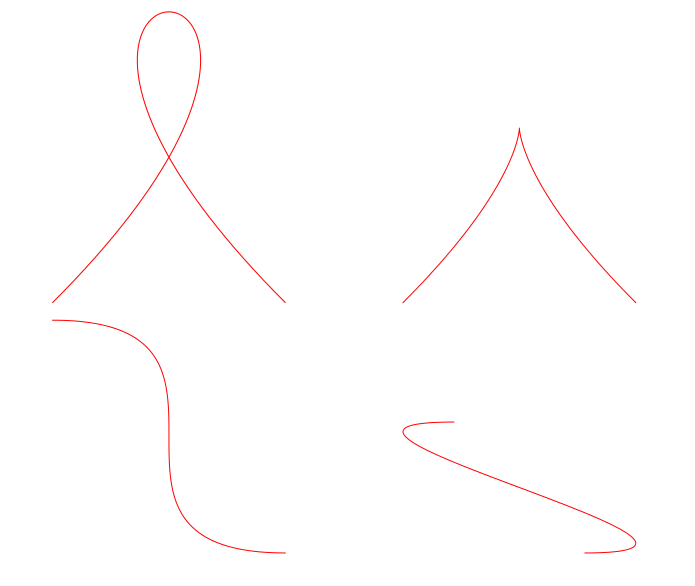
\includegraphics[max size={\textwidth}{\textheight}]{Exercise 2_files/Exercise 2_1_0.png}
    \par
    \end{center}
    
            \end{InvisibleVerbatim}
            
        
    


    % Make sure that atleast 4 lines are below the HR
    \needspace{4\baselineskip}

    
        \vspace{6pt}
        \makebox[0.1\linewidth]{\smaller\hfill\tt\color{nbframe-in-prompt}In\hspace{4pt}{[}46{]}:\hspace{4pt}}\\*
        \vspace{-2.65\baselineskip}
        \begin{ColorVerbatim}
            \vspace{-0.7\baselineskip}
            \begin{Verbatim}[commandchars=\\\{\}]
\PY{o}{\PYZpc{}}\PY{k}{matplotlib} \PY{n}{inline}
\PY{k+kn}{import} \PY{n+nn}{numpy}
\PY{k+kn}{import} \PY{n+nn}{numpy} \PY{k+kn}{as} \PY{n+nn}{np}
\PY{k+kn}{import} \PY{n+nn}{pylab}
\PY{k+kn}{import} \PY{n+nn}{matplotlib.pyplot} \PY{k+kn}{as} \PY{n+nn}{plt}

\PY{k}{class} \PY{n+nc}{HermiteCurve}\PY{p}{:}
    
    \PY{k}{def} \PY{n+nf}{\PYZus{}\PYZus{}init\PYZus{}\PYZus{}}\PY{p}{(}\PY{n+nb+bp}{self}\PY{p}{)}\PY{p}{:}
        \PY{n+nb+bp}{self}\PY{o}{.}\PY{n}{p0} \PY{o}{=} \PY{n}{np}\PY{o}{.}\PY{n}{array}\PY{p}{(}\PY{p}{[}\PY{l+m+mi}{0}\PY{p}{,} \PY{l+m+mi}{0}\PY{p}{]}\PY{p}{)}
        \PY{n+nb+bp}{self}\PY{o}{.}\PY{n}{p1} \PY{o}{=} \PY{n}{np}\PY{o}{.}\PY{n}{array}\PY{p}{(}\PY{p}{[}\PY{l+m+mi}{0}\PY{p}{,} \PY{l+m+mi}{0}\PY{p}{]}\PY{p}{)}
        \PY{n+nb+bp}{self}\PY{o}{.}\PY{n}{p0\PYZus{}tangent} \PY{o}{=} \PY{n}{np}\PY{o}{.}\PY{n}{array}\PY{p}{(}\PY{p}{[}\PY{l+m+mi}{0}\PY{p}{,} \PY{l+m+mi}{0}\PY{p}{]}\PY{p}{)}
        \PY{n+nb+bp}{self}\PY{o}{.}\PY{n}{p1\PYZus{}tangent} \PY{o}{=} \PY{n}{np}\PY{o}{.}\PY{n}{array}\PY{p}{(}\PY{p}{[}\PY{l+m+mi}{0}\PY{p}{,} \PY{l+m+mi}{0}\PY{p}{]}\PY{p}{)}
        \PY{n+nb+bp}{self}\PY{o}{.}\PY{n}{plt} \PY{o}{=} \PY{n}{plt}
        
        \PY{n+nb+bp}{self}\PY{o}{.}\PY{n}{calculcate\PYZus{}coefficients}\PY{p}{(}\PY{p}{)}
        \PY{n+nb+bp}{self}\PY{o}{.}\PY{n}{setup\PYZus{}plot}\PY{p}{(}\PY{p}{)}
        
    \PY{k}{def} \PY{n+nf}{setup\PYZus{}plot}\PY{p}{(}\PY{n+nb+bp}{self}\PY{p}{)}\PY{p}{:}
        \PY{n+nb+bp}{self}\PY{o}{.}\PY{n}{plt}\PY{o}{.}\PY{n}{margins}\PY{p}{(}\PY{l+m+mf}{0.1}\PY{p}{)}
        \PY{n+nb+bp}{self}\PY{o}{.}\PY{n}{plt}\PY{o}{.}\PY{n}{grid}\PY{p}{(}\PY{p}{)}
        
    \PY{k}{def} \PY{n+nf}{calculcate\PYZus{}coefficients}\PY{p}{(}\PY{n+nb+bp}{self}\PY{p}{)}\PY{p}{:}
        \PY{n+nb+bp}{self}\PY{o}{.}\PY{n}{a} \PY{o}{=} \PY{l+m+mi}{2} \PY{o}{*} \PY{n+nb+bp}{self}\PY{o}{.}\PY{n}{p0} \PY{o}{\PYZhy{}} \PY{l+m+mi}{2} \PY{o}{*} \PY{n+nb+bp}{self}\PY{o}{.}\PY{n}{p1} \PY{o}{+} \PY{n+nb+bp}{self}\PY{o}{.}\PY{n}{p0\PYZus{}tangent} \PY{o}{+} \PY{n+nb+bp}{self}\PY{o}{.}\PY{n}{p1\PYZus{}tangent}
        \PY{n+nb+bp}{self}\PY{o}{.}\PY{n}{b} \PY{o}{=} \PY{o}{\PYZhy{}}\PY{l+m+mi}{3} \PY{o}{*} \PY{n+nb+bp}{self}\PY{o}{.}\PY{n}{p0} \PY{o}{+} \PY{l+m+mi}{3} \PY{o}{*} \PY{n+nb+bp}{self}\PY{o}{.}\PY{n}{p1} \PY{o}{\PYZhy{}} \PY{l+m+mi}{2} \PY{o}{*} \PY{n+nb+bp}{self}\PY{o}{.}\PY{n}{p0\PYZus{}tangent} \PY{o}{\PYZhy{}} \PY{n+nb+bp}{self}\PY{o}{.}\PY{n}{p1\PYZus{}tangent}
        \PY{n+nb+bp}{self}\PY{o}{.}\PY{n}{c} \PY{o}{=} \PY{n+nb+bp}{self}\PY{o}{.}\PY{n}{p0\PYZus{}tangent}
        \PY{n+nb+bp}{self}\PY{o}{.}\PY{n}{d} \PY{o}{=} \PY{n+nb+bp}{self}\PY{o}{.}\PY{n}{p0}
        
    \PY{k}{def} \PY{n+nf}{calculate\PYZus{}coefficient\PYZus{}matrix}\PY{p}{(}\PY{n+nb+bp}{self}\PY{p}{)}\PY{p}{:}    
        \PY{n}{coefficients} \PY{o}{=} \PY{n}{numpy}\PY{o}{.}\PY{n}{matrix}\PY{p}{(}
            \PY{p}{(}
                \PY{p}{(} \PY{l+m+mi}{2}\PY{p}{,} \PY{o}{\PYZhy{}}\PY{l+m+mi}{2}\PY{p}{,}  \PY{l+m+mi}{1}\PY{p}{,}  \PY{l+m+mi}{1}\PY{p}{)}\PY{p}{,}
                \PY{p}{(}\PY{o}{\PYZhy{}}\PY{l+m+mi}{3}\PY{p}{,}  \PY{l+m+mi}{3}\PY{p}{,} \PY{o}{\PYZhy{}}\PY{l+m+mi}{2}\PY{p}{,} \PY{o}{\PYZhy{}}\PY{l+m+mi}{1}\PY{p}{)}\PY{p}{,}
                \PY{p}{(} \PY{l+m+mi}{0}\PY{p}{,}  \PY{l+m+mi}{0}\PY{p}{,}  \PY{l+m+mi}{1}\PY{p}{,}  \PY{l+m+mi}{0}\PY{p}{)}\PY{p}{,}
                \PY{p}{(} \PY{l+m+mi}{1}\PY{p}{,}  \PY{l+m+mi}{0}\PY{p}{,}  \PY{l+m+mi}{0}\PY{p}{,}  \PY{l+m+mi}{0}\PY{p}{)}
            \PY{p}{)}
        \PY{p}{)}
        
        \PY{n}{points} \PY{o}{=} \PY{n}{numpy}\PY{o}{.}\PY{n}{matrix}\PY{p}{(}
            \PY{p}{(}
                \PY{p}{(}\PY{n+nb+bp}{self}\PY{o}{.}\PY{n}{p0}\PY{p}{)}\PY{p}{,}
                \PY{p}{(}\PY{n+nb+bp}{self}\PY{o}{.}\PY{n}{p1}\PY{p}{)}\PY{p}{,}
                \PY{p}{(}\PY{n+nb+bp}{self}\PY{o}{.}\PY{n}{p0\PYZus{}tangent}\PY{p}{)}\PY{p}{,}
                \PY{p}{(}\PY{n+nb+bp}{self}\PY{o}{.}\PY{n}{p1\PYZus{}tangent}\PY{p}{)}
            \PY{p}{)}
        \PY{p}{)}
        
        \PY{k}{return} \PY{n}{np}\PY{o}{.}\PY{n}{dot}\PY{p}{(}\PY{n}{coefficients}\PY{p}{,} \PY{n}{points}\PY{p}{)}
        
    \PY{k}{def} \PY{n+nf}{calculate\PYZus{}curve\PYZus{}point}\PY{p}{(}\PY{n+nb+bp}{self}\PY{p}{,} \PY{n}{time}\PY{p}{)}\PY{p}{:}
        \PY{k}{return} \PY{n+nb+bp}{self}\PY{o}{.}\PY{n}{a} \PY{o}{*} \PY{n}{np}\PY{o}{.}\PY{n}{power}\PY{p}{(}\PY{n}{time}\PY{p}{,} \PY{l+m+mi}{3}\PY{p}{)} \PY{o}{+} \PY{n+nb+bp}{self}\PY{o}{.}\PY{n}{b} \PY{o}{*} \PY{n}{np}\PY{o}{.}\PY{n}{power}\PY{p}{(}\PY{n}{time}\PY{p}{,} \PY{l+m+mi}{2}\PY{p}{)} \PY{o}{+} \PY{n+nb+bp}{self}\PY{o}{.}\PY{n}{c} \PY{o}{*} \PY{n}{time} \PY{o}{+} \PY{n+nb+bp}{self}\PY{o}{.}\PY{n}{d}
        
    \PY{k}{def} \PY{n+nf}{plot}\PY{p}{(}\PY{n+nb+bp}{self}\PY{p}{)}\PY{p}{:}
        \PY{c}{\PYZsh{} Plot points}
        \PY{n}{x} \PY{o}{=} \PY{p}{[}\PY{n+nb+bp}{self}\PY{o}{.}\PY{n}{p0}\PY{p}{[}\PY{l+m+mi}{0}\PY{p}{]}\PY{p}{,} \PY{n+nb+bp}{self}\PY{o}{.}\PY{n}{p1}\PY{p}{[}\PY{l+m+mi}{0}\PY{p}{]}\PY{p}{]}
        \PY{n}{y} \PY{o}{=} \PY{p}{[}\PY{n+nb+bp}{self}\PY{o}{.}\PY{n}{p0}\PY{p}{[}\PY{l+m+mi}{1}\PY{p}{]}\PY{p}{,} \PY{n+nb+bp}{self}\PY{o}{.}\PY{n}{p1}\PY{p}{[}\PY{l+m+mi}{1}\PY{p}{]}\PY{p}{]}
        \PY{c}{\PYZsh{} Plot arrow}
        \PY{n}{plt}\PY{o}{.}\PY{n}{arrow}\PY{p}{(}
            \PY{n+nb+bp}{self}\PY{o}{.}\PY{n}{p0}\PY{p}{[}\PY{l+m+mi}{0}\PY{p}{]}\PY{p}{,} 
            \PY{n+nb+bp}{self}\PY{o}{.}\PY{n}{p0}\PY{p}{[}\PY{l+m+mi}{1}\PY{p}{]}\PY{p}{,} 
            \PY{n+nb+bp}{self}\PY{o}{.}\PY{n}{p0\PYZus{}tangent}\PY{p}{[}\PY{l+m+mi}{0}\PY{p}{]} \PY{o}{\PYZhy{}} \PY{n+nb+bp}{self}\PY{o}{.}\PY{n}{p0}\PY{p}{[}\PY{l+m+mi}{0}\PY{p}{]}\PY{p}{,} 
            \PY{n+nb+bp}{self}\PY{o}{.}\PY{n}{p0\PYZus{}tangent}\PY{p}{[}\PY{l+m+mi}{1}\PY{p}{]} \PY{o}{\PYZhy{}} \PY{n+nb+bp}{self}\PY{o}{.}\PY{n}{p0}\PY{p}{[}\PY{l+m+mi}{1}\PY{p}{]}
        \PY{p}{)}
        \PY{n}{plt}\PY{o}{.}\PY{n}{arrow}\PY{p}{(}
            \PY{n+nb+bp}{self}\PY{o}{.}\PY{n}{p1}\PY{p}{[}\PY{l+m+mi}{0}\PY{p}{]}\PY{p}{,}
            \PY{n+nb+bp}{self}\PY{o}{.}\PY{n}{p1}\PY{p}{[}\PY{l+m+mi}{1}\PY{p}{]}\PY{p}{,}
            \PY{n+nb+bp}{self}\PY{o}{.}\PY{n}{p1\PYZus{}tangent}\PY{p}{[}\PY{l+m+mi}{0}\PY{p}{]} \PY{o}{\PYZhy{}} \PY{n+nb+bp}{self}\PY{o}{.}\PY{n}{p1}\PY{p}{[}\PY{l+m+mi}{0}\PY{p}{]}\PY{p}{,}
            \PY{n+nb+bp}{self}\PY{o}{.}\PY{n}{p1\PYZus{}tangent}\PY{p}{[}\PY{l+m+mi}{1}\PY{p}{]} \PY{o}{\PYZhy{}} \PY{n+nb+bp}{self}\PY{o}{.}\PY{n}{p1}\PY{p}{[}\PY{l+m+mi}{1}\PY{p}{]}
        \PY{p}{)}
        \PY{n}{plt}\PY{o}{.}\PY{n}{plot}\PY{p}{(}\PY{n}{x}\PY{p}{,} \PY{n}{y}\PY{p}{,} \PY{l+s}{\PYZsq{}}\PY{l+s}{ro}\PY{l+s}{\PYZsq{}}\PY{p}{)}
        
        \PY{c}{\PYZsh{} Prepare data}
        \PY{n+nb+bp}{self}\PY{o}{.}\PY{n}{calculcate\PYZus{}coefficients}\PY{p}{(}\PY{p}{)}
        \PY{n}{coeff\PYZus{}matrix} \PY{o}{=} \PY{n+nb+bp}{self}\PY{o}{.}\PY{n}{calculate\PYZus{}coefficient\PYZus{}matrix}\PY{p}{(}\PY{p}{)}
        
        \PY{c}{\PYZsh{} Gather data}
        \PY{n}{plot\PYZus{}data} \PY{o}{=} \PY{p}{[}\PY{p}{]}
        \PY{k}{for} \PY{n}{t} \PY{o+ow}{in} \PY{n}{numpy}\PY{o}{.}\PY{n}{linspace}\PY{p}{(}\PY{l+m+mi}{0}\PY{p}{,} \PY{l+m+mi}{1}\PY{p}{,} \PY{l+m+mi}{100}\PY{p}{)}\PY{p}{:}
            \PY{n}{plot\PYZus{}data}\PY{o}{.}\PY{n}{append}\PY{p}{(}
                \PY{n}{numpy}\PY{o}{.}\PY{n}{dot}\PY{p}{(}
                    \PY{n}{numpy}\PY{o}{.}\PY{n}{matrix}\PY{p}{(}
                        \PY{p}{(}
                            \PY{p}{(}\PY{n}{numpy}\PY{o}{.}\PY{n}{power}\PY{p}{(}\PY{n}{t}\PY{p}{,} \PY{l+m+mi}{3}\PY{p}{)}\PY{p}{)}\PY{p}{,}
                            \PY{p}{(}\PY{n}{numpy}\PY{o}{.}\PY{n}{power}\PY{p}{(}\PY{n}{t}\PY{p}{,} \PY{l+m+mi}{2}\PY{p}{)}\PY{p}{)}\PY{p}{,}
                            \PY{p}{(}\PY{n}{t}\PY{p}{)}\PY{p}{,}
                            \PY{p}{(}\PY{l+m+mi}{1}\PY{p}{)}
                        \PY{p}{)}
                    \PY{p}{)}\PY{p}{,}
                    \PY{n}{coeff\PYZus{}matrix}
                \PY{p}{)}
            \PY{p}{)}
        
        \PY{n}{x} \PY{o}{=} \PY{p}{[}\PY{p}{]}
        \PY{n}{y} \PY{o}{=} \PY{p}{[}\PY{p}{]}
        \PY{k}{for} \PY{n}{data} \PY{o+ow}{in} \PY{n}{plot\PYZus{}data}\PY{p}{:}
            \PY{n}{x}\PY{o}{.}\PY{n}{append}\PY{p}{(}\PY{n}{data}\PY{o}{.}\PY{n}{A}\PY{p}{[}\PY{l+m+mi}{0}\PY{p}{]}\PY{p}{[}\PY{l+m+mi}{0}\PY{p}{]}\PY{p}{)}
            \PY{n}{y}\PY{o}{.}\PY{n}{append}\PY{p}{(}\PY{n}{data}\PY{o}{.}\PY{n}{A}\PY{p}{[}\PY{l+m+mi}{0}\PY{p}{]}\PY{p}{[}\PY{l+m+mi}{1}\PY{p}{]}\PY{p}{)}
            
        \PY{c}{\PYZsh{} Plot}
        \PY{n}{plt}\PY{o}{.}\PY{n}{plot}\PY{p}{(}\PY{n}{x}\PY{p}{,} \PY{n}{y}\PY{p}{)}
        
\end{Verbatim}

            
                \vspace{-0.2\baselineskip}
            
        \end{ColorVerbatim}
    


    % Make sure that atleast 4 lines are below the HR
    \needspace{4\baselineskip}

    
        \vspace{6pt}
        \makebox[0.1\linewidth]{\smaller\hfill\tt\color{nbframe-in-prompt}In\hspace{4pt}{[}9{]}:\hspace{4pt}}\\*
        \vspace{-2.65\baselineskip}
        \begin{ColorVerbatim}
            \vspace{-0.7\baselineskip}
            \begin{Verbatim}[commandchars=\\\{\}]
\PY{c}{\PYZsh{} Just some test..}

\PY{n}{c} \PY{o}{=} \PY{n}{HermiteCurve}\PY{p}{(}\PY{p}{)}
\PY{c}{\PYZsh{} P0}
\PY{n}{c}\PY{o}{.}\PY{n}{p0} \PY{o}{=} \PY{n}{np}\PY{o}{.}\PY{n}{array}\PY{p}{(}\PY{p}{[}\PY{l+m+mi}{0}\PY{p}{,} \PY{l+m+mi}{0}\PY{p}{]}\PY{p}{)}
\PY{n}{c}\PY{o}{.}\PY{n}{p0\PYZus{}tangent} \PY{o}{=} \PY{n}{np}\PY{o}{.}\PY{n}{array}\PY{p}{(}\PY{p}{[}\PY{o}{\PYZhy{}}\PY{l+m+mf}{0.25}\PY{p}{,} \PY{l+m+mf}{0.5}\PY{p}{]}\PY{p}{)}

\PY{c}{\PYZsh{} P1}
\PY{n}{c}\PY{o}{.}\PY{n}{p1} \PY{o}{=} \PY{n}{np}\PY{o}{.}\PY{n}{array}\PY{p}{(}\PY{p}{[}\PY{l+m+mi}{1}\PY{p}{,} \PY{l+m+mi}{1}\PY{p}{]}\PY{p}{)}
\PY{n}{c}\PY{o}{.}\PY{n}{p1\PYZus{}tangent} \PY{o}{=} \PY{n}{np}\PY{o}{.}\PY{n}{array}\PY{p}{(}\PY{p}{[}\PY{l+m+mf}{1.1}\PY{p}{,} \PY{l+m+mf}{0.2}\PY{p}{]}\PY{p}{)}

\PY{n}{c}\PY{o}{.}\PY{n}{plot}\PY{p}{(}\PY{p}{)}
\end{Verbatim}

            
                \vspace{-0.2\baselineskip}
            
        \end{ColorVerbatim}
    

    

        % If the first block is an image, minipage the image.  Else
        % request a certain amount of space for the input text.
        \needspace{4\baselineskip}
        
        

            % Add document contents.
            
                \begin{InvisibleVerbatim}
                \vspace{-0.5\baselineskip}
    \begin{center}
    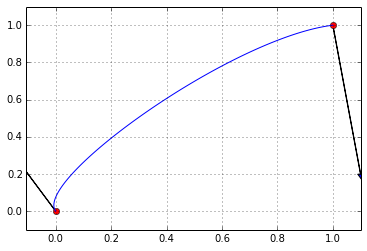
\includegraphics[max size={\textwidth}{\textheight}]{Exercise 2_files/Exercise 2_3_0.png}
    \par
    \end{center}
    
            \end{InvisibleVerbatim}
            
        
    


    % Make sure that atleast 4 lines are below the HR
    \needspace{4\baselineskip}

    
        \vspace{6pt}
        \makebox[0.1\linewidth]{\smaller\hfill\tt\color{nbframe-in-prompt}In\hspace{4pt}{[}10{]}:\hspace{4pt}}\\*
        \vspace{-2.65\baselineskip}
        \begin{ColorVerbatim}
            \vspace{-0.7\baselineskip}
            \begin{Verbatim}[commandchars=\\\{\}]
\PY{c}{\PYZsh{} Here we go.. 2.1}
\PY{n}{c} \PY{o}{=} \PY{n}{HermiteCurve}\PY{p}{(}\PY{p}{)}
\PY{c}{\PYZsh{} P0}
\PY{n}{c}\PY{o}{.}\PY{n}{p0} \PY{o}{=} \PY{n}{np}\PY{o}{.}\PY{n}{array}\PY{p}{(}\PY{p}{[}\PY{l+m+mi}{0}\PY{p}{,} \PY{l+m+mi}{0}\PY{p}{]}\PY{p}{)}
\PY{n}{c}\PY{o}{.}\PY{n}{p0\PYZus{}tangent} \PY{o}{=} \PY{n}{np}\PY{o}{.}\PY{n}{array}\PY{p}{(}\PY{p}{[}\PY{l+m+mf}{100.3}\PY{p}{,} \PY{l+m+mf}{1.2}\PY{p}{]}\PY{p}{)}

\PY{c}{\PYZsh{} P1}
\PY{n}{c}\PY{o}{.}\PY{n}{p1} \PY{o}{=} \PY{n}{np}\PY{o}{.}\PY{n}{array}\PY{p}{(}\PY{p}{[}\PY{l+m+mi}{1}\PY{p}{,} \PY{l+m+mi}{0}\PY{p}{]}\PY{p}{)}
\PY{n}{c}\PY{o}{.}\PY{n}{p1\PYZus{}tangent} \PY{o}{=} \PY{n}{np}\PY{o}{.}\PY{n}{array}\PY{p}{(}\PY{p}{[}\PY{l+m+mf}{100.3}\PY{p}{,} \PY{o}{\PYZhy{}}\PY{l+m+mf}{1.2}\PY{p}{]}\PY{p}{)}

\PY{n}{c}\PY{o}{.}\PY{n}{plot}\PY{p}{(}\PY{p}{)}
\end{Verbatim}

            
                \vspace{-0.2\baselineskip}
            
        \end{ColorVerbatim}
    

    

        % If the first block is an image, minipage the image.  Else
        % request a certain amount of space for the input text.
        \needspace{4\baselineskip}
        
        

            % Add document contents.
            
                \begin{InvisibleVerbatim}
                \vspace{-0.5\baselineskip}
    \begin{center}
    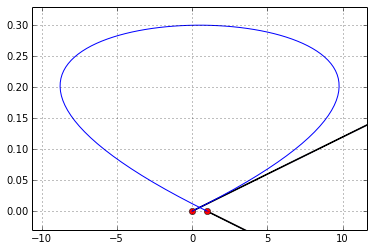
\includegraphics[max size={\textwidth}{\textheight}]{Exercise 2_files/Exercise 2_4_0.png}
    \par
    \end{center}
    
            \end{InvisibleVerbatim}
            
        
    


    % Make sure that atleast 4 lines are below the HR
    \needspace{4\baselineskip}

    
        \vspace{6pt}
        \makebox[0.1\linewidth]{\smaller\hfill\tt\color{nbframe-in-prompt}In\hspace{4pt}{[}11{]}:\hspace{4pt}}\\*
        \vspace{-2.65\baselineskip}
        \begin{ColorVerbatim}
            \vspace{-0.7\baselineskip}
            \begin{Verbatim}[commandchars=\\\{\}]
\PY{c}{\PYZsh{} Here we go.. 2.3}
\PY{n}{c} \PY{o}{=} \PY{n}{HermiteCurve}\PY{p}{(}\PY{p}{)}
\PY{c}{\PYZsh{} P0}
\PY{n}{c}\PY{o}{.}\PY{n}{p0} \PY{o}{=} \PY{n}{np}\PY{o}{.}\PY{n}{array}\PY{p}{(}\PY{p}{[}\PY{l+m+mi}{0}\PY{p}{,} \PY{l+m+mi}{1}\PY{p}{]}\PY{p}{)}
\PY{n}{c}\PY{o}{.}\PY{n}{p0\PYZus{}tangent} \PY{o}{=} \PY{n}{np}\PY{o}{.}\PY{n}{array}\PY{p}{(}\PY{p}{[}\PY{l+m+mi}{3}\PY{p}{,} \PY{l+m+mf}{0.1}\PY{p}{]}\PY{p}{)}

\PY{c}{\PYZsh{} P1}
\PY{n}{c}\PY{o}{.}\PY{n}{p1} \PY{o}{=} \PY{n}{np}\PY{o}{.}\PY{n}{array}\PY{p}{(}\PY{p}{[}\PY{l+m+mi}{1}\PY{p}{,} \PY{l+m+mi}{0}\PY{p}{]}\PY{p}{)}
\PY{n}{c}\PY{o}{.}\PY{n}{p1\PYZus{}tangent} \PY{o}{=} \PY{n}{np}\PY{o}{.}\PY{n}{array}\PY{p}{(}\PY{p}{[}\PY{l+m+mi}{3}\PY{p}{,} \PY{o}{\PYZhy{}}\PY{l+m+mf}{0.2}\PY{p}{]}\PY{p}{)}

\PY{n}{c}\PY{o}{.}\PY{n}{plot}\PY{p}{(}\PY{p}{)}
\end{Verbatim}

            
                \vspace{-0.2\baselineskip}
            
        \end{ColorVerbatim}
    

    

        % If the first block is an image, minipage the image.  Else
        % request a certain amount of space for the input text.
        \needspace{4\baselineskip}
        
        

            % Add document contents.
            
                \begin{InvisibleVerbatim}
                \vspace{-0.5\baselineskip}
    \begin{center}
    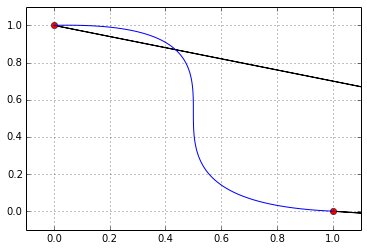
\includegraphics[max size={\textwidth}{\textheight}]{Exercise 2_files/Exercise 2_5_0.png}
    \par
    \end{center}
    
            \end{InvisibleVerbatim}
            
        
    


    % Make sure that atleast 4 lines are below the HR
    \needspace{4\baselineskip}

    
        \vspace{6pt}
        \makebox[0.1\linewidth]{\smaller\hfill\tt\color{nbframe-in-prompt}In\hspace{4pt}{[}34{]}:\hspace{4pt}}\\*
        \vspace{-2.65\baselineskip}
        \begin{ColorVerbatim}
            \vspace{-0.7\baselineskip}
            \begin{Verbatim}[commandchars=\\\{\}]
\PY{c}{\PYZsh{} Here we go.. 2.4}
\PY{n}{c} \PY{o}{=} \PY{n}{HermiteCurve}\PY{p}{(}\PY{p}{)}
\PY{c}{\PYZsh{} P0}
\PY{n}{c}\PY{o}{.}\PY{n}{p0} \PY{o}{=} \PY{n}{np}\PY{o}{.}\PY{n}{array}\PY{p}{(}\PY{p}{[}\PY{l+m+mi}{0}\PY{p}{,} \PY{l+m+mi}{1}\PY{p}{]}\PY{p}{)}
\PY{n}{c}\PY{o}{.}\PY{n}{p0\PYZus{}tangent} \PY{o}{=} \PY{n}{np}\PY{o}{.}\PY{n}{array}\PY{p}{(}\PY{p}{[}\PY{o}{\PYZhy{}}\PY{l+m+mi}{3}\PY{p}{,} \PY{l+m+mf}{0.1}\PY{p}{]}\PY{p}{)}

\PY{c}{\PYZsh{} P1}
\PY{n}{c}\PY{o}{.}\PY{n}{p1} \PY{o}{=} \PY{n}{np}\PY{o}{.}\PY{n}{array}\PY{p}{(}\PY{p}{[}\PY{l+m+mi}{1}\PY{p}{,} \PY{l+m+mi}{0}\PY{p}{]}\PY{p}{)}
\PY{n}{c}\PY{o}{.}\PY{n}{p1\PYZus{}tangent} \PY{o}{=} \PY{n}{np}\PY{o}{.}\PY{n}{array}\PY{p}{(}\PY{p}{[}\PY{o}{\PYZhy{}}\PY{l+m+mi}{3}\PY{p}{,} \PY{o}{\PYZhy{}}\PY{l+m+mf}{0.1}\PY{p}{]}\PY{p}{)}

\PY{n}{c}\PY{o}{.}\PY{n}{plot}\PY{p}{(}\PY{p}{)}
\end{Verbatim}

            
                \vspace{-0.2\baselineskip}
            
        \end{ColorVerbatim}
    

    

        % If the first block is an image, minipage the image.  Else
        % request a certain amount of space for the input text.
        \needspace{4\baselineskip}
        
        

            % Add document contents.
            
                \begin{InvisibleVerbatim}
                \vspace{-0.5\baselineskip}
    \begin{center}
    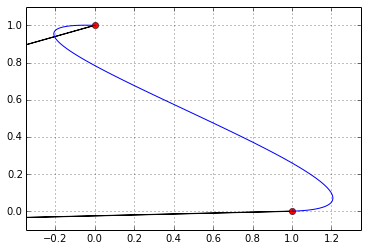
\includegraphics[max size={\textwidth}{\textheight}]{Exercise 2_files/Exercise 2_6_0.png}
    \par
    \end{center}
    
            \end{InvisibleVerbatim}
            
        
    


    % Make sure that atleast 4 lines are below the HR
    \needspace{4\baselineskip}

    
        \vspace{6pt}
        \makebox[0.1\linewidth]{\smaller\hfill\tt\color{nbframe-in-prompt}In\hspace{4pt}{[}38{]}:\hspace{4pt}}\\*
        \vspace{-2.65\baselineskip}
        \begin{ColorVerbatim}
            \vspace{-0.7\baselineskip}
            \begin{Verbatim}[commandchars=\\\{\}]
\PY{c}{\PYZsh{} Here we go.. 4}
\PY{n}{c} \PY{o}{=} \PY{n}{HermiteCurve}\PY{p}{(}\PY{p}{)}
\PY{c}{\PYZsh{} P0}
\PY{n}{c}\PY{o}{.}\PY{n}{p0} \PY{o}{=} \PY{n}{np}\PY{o}{.}\PY{n}{array}\PY{p}{(}\PY{p}{[}\PY{l+m+mf}{0.8}\PY{p}{,} \PY{l+m+mf}{0.2}\PY{p}{]}\PY{p}{)}
\PY{n}{c}\PY{o}{.}\PY{n}{p0\PYZus{}tangent} \PY{o}{=} \PY{n}{np}\PY{o}{.}\PY{n}{array}\PY{p}{(}\PY{p}{[}\PY{l+m+mi}{0}\PY{p}{,}\PY{l+m+mi}{0}\PY{p}{]}\PY{p}{)}

\PY{c}{\PYZsh{} P1}
\PY{n}{c}\PY{o}{.}\PY{n}{p1} \PY{o}{=} \PY{n}{np}\PY{o}{.}\PY{n}{array}\PY{p}{(}\PY{p}{[}\PY{l+m+mf}{0.1}\PY{p}{,} \PY{l+m+mi}{0}\PY{p}{]}\PY{p}{)}
\PY{n}{c}\PY{o}{.}\PY{n}{p1\PYZus{}tangent} \PY{o}{=} \PY{n}{np}\PY{o}{.}\PY{n}{array}\PY{p}{(}\PY{p}{[}\PY{l+m+mi}{0}\PY{p}{,}\PY{l+m+mi}{0}\PY{p}{]}\PY{p}{)}

\PY{n}{c}\PY{o}{.}\PY{n}{plot}\PY{p}{(}\PY{p}{)}
\end{Verbatim}

            
                \vspace{-0.2\baselineskip}
            
        \end{ColorVerbatim}
    

    

        % If the first block is an image, minipage the image.  Else
        % request a certain amount of space for the input text.
        \needspace{4\baselineskip}
        
        

            % Add document contents.
            
                \begin{InvisibleVerbatim}
                \vspace{-0.5\baselineskip}
    \begin{center}
    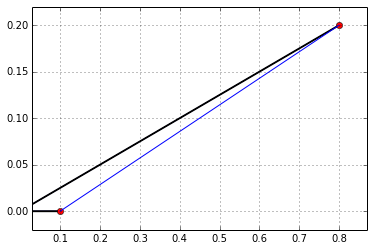
\includegraphics[max size={\textwidth}{\textheight}]{Exercise 2_files/Exercise 2_7_0.png}
    \par
    \end{center}
    
            \end{InvisibleVerbatim}
            
        
    


    % Make sure that atleast 4 lines are below the HR
    \needspace{4\baselineskip}

    
        \vspace{6pt}
        \makebox[0.1\linewidth]{\smaller\hfill\tt\color{nbframe-in-prompt}In\hspace{4pt}{[}51{]}:\hspace{4pt}}\\*
        \vspace{-2.65\baselineskip}
        \begin{ColorVerbatim}
            \vspace{-0.7\baselineskip}
            \begin{Verbatim}[commandchars=\\\{\}]
\PY{c}{\PYZsh{} Here we go.. 5}
\PY{n}{c} \PY{o}{=} \PY{n}{HermiteCurve}\PY{p}{(}\PY{p}{)}
\PY{c}{\PYZsh{} P0}
\PY{n}{c}\PY{o}{.}\PY{n}{p0} \PY{o}{=} \PY{n}{np}\PY{o}{.}\PY{n}{array}\PY{p}{(}\PY{p}{[}\PY{l+m+mi}{0}\PY{p}{,} \PY{l+m+mi}{0}\PY{p}{]}\PY{p}{)}
\PY{n}{c}\PY{o}{.}\PY{n}{p0\PYZus{}tangent} \PY{o}{=} \PY{n}{np}\PY{o}{.}\PY{n}{array}\PY{p}{(}\PY{p}{[}\PY{l+m+mi}{1}\PY{p}{,}\PY{l+m+mi}{0}\PY{p}{]}\PY{p}{)}

\PY{c}{\PYZsh{} P1}
\PY{n}{c}\PY{o}{.}\PY{n}{p1} \PY{o}{=} \PY{n}{np}\PY{o}{.}\PY{n}{array}\PY{p}{(}\PY{p}{[}\PY{l+m+mi}{1}\PY{p}{,} \PY{l+m+mi}{1}\PY{p}{]}\PY{p}{)}
\PY{n}{c}\PY{o}{.}\PY{n}{p1\PYZus{}tangent} \PY{o}{=} \PY{n}{np}\PY{o}{.}\PY{n}{array}\PY{p}{(}\PY{p}{[}\PY{l+m+mi}{0}\PY{p}{,}\PY{l+m+mi}{1}\PY{p}{]}\PY{p}{)}

\PY{n}{c}\PY{o}{.}\PY{n}{plot}\PY{p}{(}\PY{p}{)}

\PY{n}{c2} \PY{o}{=} \PY{n}{HermiteCurve}\PY{p}{(}\PY{p}{)}
\PY{c}{\PYZsh{} P1}
\PY{n}{c2}\PY{o}{.}\PY{n}{p0} \PY{o}{=} \PY{n}{np}\PY{o}{.}\PY{n}{array}\PY{p}{(}\PY{p}{[}\PY{l+m+mi}{1}\PY{p}{,} \PY{l+m+mi}{1}\PY{p}{]}\PY{p}{)}
\PY{n}{c2}\PY{o}{.}\PY{n}{p0\PYZus{}tangent} \PY{o}{=} \PY{n}{np}\PY{o}{.}\PY{n}{array}\PY{p}{(}\PY{p}{[}\PY{l+m+mi}{0}\PY{p}{,}\PY{l+m+mi}{1}\PY{p}{]}\PY{p}{)}

\PY{c}{\PYZsh{} P2}
\PY{n}{c2}\PY{o}{.}\PY{n}{p1} \PY{o}{=} \PY{n}{np}\PY{o}{.}\PY{n}{array}\PY{p}{(}\PY{p}{[}\PY{l+m+mi}{0}\PY{p}{,} \PY{l+m+mi}{2}\PY{p}{]}\PY{p}{)}
\PY{n}{c2}\PY{o}{.}\PY{n}{p1\PYZus{}tangent} \PY{o}{=} \PY{n}{np}\PY{o}{.}\PY{n}{array}\PY{p}{(}\PY{p}{[}\PY{o}{\PYZhy{}}\PY{l+m+mi}{1}\PY{p}{,}\PY{l+m+mi}{0}\PY{p}{]}\PY{p}{)}

\PY{n}{c2}\PY{o}{.}\PY{n}{plot}\PY{p}{(}\PY{p}{)}

\PY{n}{c3} \PY{o}{=} \PY{n}{HermiteCurve}\PY{p}{(}\PY{p}{)}
\PY{c}{\PYZsh{} P2}
\PY{n}{c3}\PY{o}{.}\PY{n}{p0} \PY{o}{=} \PY{n}{np}\PY{o}{.}\PY{n}{array}\PY{p}{(}\PY{p}{[}\PY{l+m+mi}{0}\PY{p}{,} \PY{l+m+mi}{2}\PY{p}{]}\PY{p}{)}
\PY{n}{c3}\PY{o}{.}\PY{n}{p0\PYZus{}tangent} \PY{o}{=} \PY{n}{np}\PY{o}{.}\PY{n}{array}\PY{p}{(}\PY{p}{[}\PY{o}{\PYZhy{}}\PY{l+m+mi}{1}\PY{p}{,}\PY{l+m+mi}{0}\PY{p}{]}\PY{p}{)}

\PY{c}{\PYZsh{} P3}
\PY{n}{c3}\PY{o}{.}\PY{n}{p1} \PY{o}{=} \PY{n}{np}\PY{o}{.}\PY{n}{array}\PY{p}{(}\PY{p}{[}\PY{o}{\PYZhy{}}\PY{l+m+mi}{1}\PY{p}{,} \PY{l+m+mi}{1}\PY{p}{]}\PY{p}{)}
\PY{n}{c3}\PY{o}{.}\PY{n}{p1\PYZus{}tangent} \PY{o}{=} \PY{n}{np}\PY{o}{.}\PY{n}{array}\PY{p}{(}\PY{p}{[}\PY{l+m+mi}{0}\PY{p}{,}\PY{o}{\PYZhy{}}\PY{l+m+mi}{1}\PY{p}{]}\PY{p}{)}

\PY{n}{c3}\PY{o}{.}\PY{n}{plot}\PY{p}{(}\PY{p}{)}

\PY{k}{for} \PY{n}{u} \PY{o+ow}{in} \PY{n}{numpy}\PY{o}{.}\PY{n}{arange}\PY{p}{(}\PY{l+m+mi}{0}\PY{p}{,} \PY{l+m+mi}{1}\PY{p}{,} \PY{l+m+mf}{0.2}\PY{p}{)}\PY{p}{:}
    \PY{k}{print} \PY{l+s}{\PYZdq{}}\PY{l+s}{Curve 0 at \PYZob{}0\PYZcb{}: \PYZob{}1\PYZcb{}}\PY{l+s}{\PYZdq{}}\PY{o}{.}\PY{n}{format}\PY{p}{(}\PY{n}{u}\PY{p}{,} \PY{n}{c}\PY{o}{.}\PY{n}{calculate\PYZus{}curve\PYZus{}point}\PY{p}{(}\PY{n}{u}\PY{p}{)}\PY{p}{)}
    \PY{k}{print} \PY{l+s}{\PYZdq{}}\PY{l+s}{Curve 1 at \PYZob{}0\PYZcb{}: \PYZob{}1\PYZcb{}}\PY{l+s}{\PYZdq{}}\PY{o}{.}\PY{n}{format}\PY{p}{(}\PY{n}{u}\PY{p}{,} \PY{n}{c2}\PY{o}{.}\PY{n}{calculate\PYZus{}curve\PYZus{}point}\PY{p}{(}\PY{n}{u}\PY{p}{)}\PY{p}{)}
    \PY{k}{print} \PY{l+s}{\PYZdq{}}\PY{l+s}{Curve 2 at \PYZob{}0\PYZcb{}: \PYZob{}1\PYZcb{}}\PY{l+s}{\PYZdq{}}\PY{o}{.}\PY{n}{format}\PY{p}{(}\PY{n}{u}\PY{p}{,} \PY{n}{c3}\PY{o}{.}\PY{n}{calculate\PYZus{}curve\PYZus{}point}\PY{p}{(}\PY{n}{u}\PY{p}{)}\PY{p}{)}
    \PY{k}{print} \PY{l+s}{\PYZdq{}}\PY{l+s}{\PYZdq{}}
\end{Verbatim}

            
                \vspace{-0.2\baselineskip}
            
        \end{ColorVerbatim}
    

    

        % If the first block is an image, minipage the image.  Else
        % request a certain amount of space for the input text.
        \needspace{4\baselineskip}
        
        

            % Add document contents.
            
                \begin{InvisibleVerbatim}
                \vspace{-0.5\baselineskip}
\begin{alltt}Curve 0 at 0.0: [ 0.  0.]
Curve 1 at 0.0: [ 1.  1.]
Curve 2 at 0.0: [ 0.  2.]

Curve 0 at 0.2: [ 0.232  0.072]
Curve 1 at 0.2: [ 0.928  1.232]
Curve 2 at 0.2: [-0.232  1.928]

Curve 0 at 0.4: [ 0.496  0.256]
Curve 1 at 0.4: [ 0.744  1.496]
Curve 2 at 0.4: [-0.496  1.744]

Curve 0 at 0.6: [ 0.744  0.504]
Curve 1 at 0.6: [ 0.496  1.744]
Curve 2 at 0.6: [-0.744  1.496]

Curve 0 at 0.8: [ 0.928  0.768]
Curve 1 at 0.8: [ 0.232  1.928]
Curve 2 at 0.8: [-0.928  1.232]

\end{alltt}

            \end{InvisibleVerbatim}
            
                \begin{InvisibleVerbatim}
                \vspace{-0.5\baselineskip}
    \begin{center}
    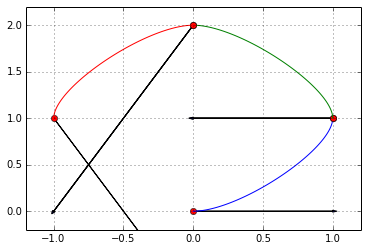
\includegraphics[max size={\textwidth}{\textheight}]{Exercise 2_files/Exercise 2_8_1.png}
    \par
    \end{center}
    
            \end{InvisibleVerbatim}
            
        
    


    % Make sure that atleast 4 lines are below the HR
    \needspace{4\baselineskip}

    
        \vspace{6pt}
        \makebox[0.1\linewidth]{\smaller\hfill\tt\color{nbframe-in-prompt}In\hspace{4pt}{[}{]}:\hspace{4pt}}\\*
        \vspace{-2.65\baselineskip}
        \begin{ColorVerbatim}
            \vspace{-0.7\baselineskip}
            \begin{Verbatim}[commandchars=\\\{\}]

\end{Verbatim}

            
                \vspace{0.3\baselineskip}
            
        \end{ColorVerbatim}
    

        

        \renewcommand{\indexname}{Index}
        \printindex

    % End of document
    \end{document}


